\newpage
\changeindent{0cm}
\section{要素技術}
\label{sec:tech}
\changeindent{2cm}

% TODO
% - DARTSの説明 論文を見ながらLoss, w* などの補足を増やす
% - TDGAの説明 自分の言葉に置き換える and 拡張した部分+エントロピー部分の説明

%9-12
本章では,本研究の提案手法に用いた技術について説明する.

%LSTM
\changeindent{0cm}
\subsection{Neural Architecture Search}
\changeindent{2cm}
\label{sec:02_deep}
本章では本研究で用いたDifferentiable Architecture Search(DARTS)をはじめとした
Neural Architecture Search(NAS) について説明する.

従来の機械学習では手作業によって設計されたモデルをデータセットで学習し重みを最適化するが,
ニューラルネットワークの設計は直感的でなく,
チューニングに人による労力を多く必要とするため,
ニューラルネットワークの設計は非常に困難である.
NAS は機械学習の分野で使用されているニューラルネットワークの設計を自動化する手法である.


\changeindent{0cm}
\subsubsection{Neural Architecture Search with Reinforcement Learning}
\changeindent{2cm}
\label{sec:02_nas}
Neural Architecture Search with Reinforcement Learning(NAS with RL)\cite{DBLP:journals/corr/ZophL16}は,
ニューラルネットワークが構造に関する設定の文字列で表現できることを利用して,
この文字列を生成する Recurrent Neural Network(RNN)\cite{mikolov2010recurrent}を
強化学習 Reinforcement Learning(RL)\cite{sutton2018reinforcement}によって学習する.

RNNはレイヤーごとにフィルタの高さ・幅, ストライドの高さ・幅, フィルタ数を決定し,
RNNによって生成された構造は, ニューラルネットワークとしてその重みが学習され
テストの正答率によって性能が評価される.
その性能から得られた報酬で, 方策勾配法(Policy gradient method)\cite{sutton1999policy}による RNN の更新を行い,
アーキテクチャが最適化される.

NAS with RL は高い性能を達成した一方で, 計算に数千 GPU days が必要となる問題もある.

\changeindent{0cm}
\subsubsection{Differentiable Architecture Search}
\changeindent{2cm}
\label{sec:02_darts}

\begin{figure}[t]
  \begin{center}
    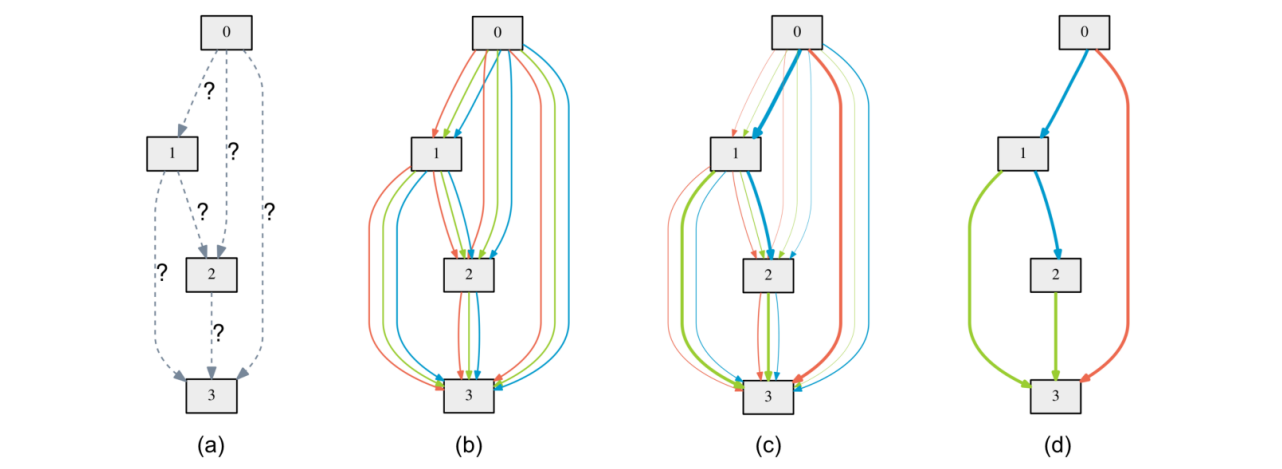
\includegraphics[clip,width=15cm]{./fig/02.tech/darts.png}
  \end{center}
  \caption{DARTS の概念図}
  (a) はじめ辺上の演算子は不明 (b) 各辺の演算子候補の混合で置換することで探索空間を連続性緩和 (c) 混合確率とネットワークの重みを最適化 (d) 学習した混合確率から最終的なアーキテクチャを導出
  (文献\cite{DBLP:journals/corr/abs-1806-09055}の 図1 参照)
  \label{fig:darts}
\end{figure}

Differentiable Architecture Search(DARTS)\cite{DBLP:journals/corr/abs-1806-09055}は,
離散的なアーキテクチャ探索空間に強化学習を適用した NAS with RL とは異なり,
微分可能な方法で定式化し\cite{Paszke2017AutomaticDI},
偏微分による勾配降下法を使用してアーキテクチャを効率的に探索する手法である.

探索空間を連続にするため, カテゴリカルな演算子の選択の代わりに, 候補全ての可能性をもつ混合演算子を
(\ref{eq:darts/operation}) 式で定義する.
アーキテクチャを有向非巡回グラフで表したとき, ノードを潜在的な特徴表現 $\bm{x}^{(i)}$,
エッジを特徴 $\bm{x}^{(i)}$ が適用される関数 $o(・)$ とすると,
\begin{equation}
  \label{eq:darts/operation}
  \bar{o}^{(i, j)}(\bm{a}) = \sum_{o \in \mathcal{O}} \frac{\exp(\bm{\alpha}^{(i, j)}_o)}{\sum_{o' \in \mathcal{O}} \exp(\bm{\alpha}^{(i, j)}_{o'})} o(\bm{x})
\end{equation}
となる. ここで
$\mathcal{O}$ は探索する演算子の候補集合,
$\bm{\alpha}^{(i, j)}$ はエッジ $(i, j)$ の混合演算子の重みベクトルである.
DARTSは勾配降下法によって連続変数集合$\bm{\alpha}$を学習する.

$\bm{\alpha}$ とレイヤーの重み $\bm{w}$ のBi-Level最適化問題\cite{Colson2007AnOO}を
$\bm{w}$ の近似によって同時に学習し,
NASにおいて 3000 GPU days 必要なタスクに対してDARTSは 3.3 GPU days まで高速化した.

DARTSでは次元を統一するためセルと呼ぶ小さなネットワーク構造を重ねたモデルを利用する.
セルを構成するノードは2つのノードからの演算子エッジを持ち,
どのノードからの演算子を選ぶのかをアーキテクチャを示す重み $\bm{\alpha}$ によって決定する.
DARTSの問題点として位置と演算子の種類は探索できるが,
大局的な構造やノードの持つエッジ数など固定されたアーキテクチャにしか適用できない点が挙げられる.


\changeindent{0cm}
\subsection{Genetic Algorithm}
\changeindent{2cm}
\label{sec:02_ga}
遺伝的アルゴリズム(Genetic Algorithm : GA)は生物の進化の仕組みを模倣した最適化手法である.
問題の解候補を遺伝子の持つ個体として表現し, 適応度によって個体を評価・選択する.
交叉・突然変異などの操作によって解候補の多様性を保ちつつ,
近傍を探索しながら世代を重ねて近似的な最適解を求める.

選択は現世代から次世代の個体群を選ぶ操作である.

トーナメント選択は, 個体群から一定数 (トーナメントサイズ) の個体をランダムに選び, 最も適応度の高いものを残す.
適応度の差は反映されないため, 偶然性が高い.


交叉は現世代から子を生成する操作である.
遺伝子型がバイナリ型, 実数型, 順序型かによってそれぞれ交叉方法が存在する.
バイナリ型では,
\begin{itemize}
  \item 1点交叉 : 染色体中の1箇所でランダムに切断し, 親の遺伝子を入れ替える
  \item 多点交叉 : 染色体中の複数箇所でランダムに切断し, 親の遺伝子を互い違いに入れ替える
  \item 一様交叉 : 遺伝子座ごとの交叉確率によって, 各遺伝子座でランダムに親の遺伝子を入れ替える
\end{itemize}
などがある.
実数型ではこれらに加えて,
\begin{itemize}
  \item BLX-$\alpha$ : 両親の遺伝子が存在する領域に$\alpha$倍した範囲から子を生成する手法. 領域の拡大によって多様性を保つ.
  \item UNDX : 正規分布に従い, 両親の周辺にその中点に対し対称な位置に2つの子を生成することで, 多様性を維持する手法.
\end{itemize}
も選択できる.

突然変異は個体をランダムに変化させる操作である.
解が収束した場合, 交叉にはない局所解からの脱出という効果を持つが,
突然変異率が高すぎるとランダム探索になるため十分に小さな値を用いる.
変異方法には, 各遺伝子座でランダムに対立遺伝子へ置き換える方法, 実数値に対して摂動を与える方法などがある.

% 初期収束問題
またGAには初期収束と呼ばれる, 探索の初期段階で適応度が高い個体だけが選択され続け,
個体群を同じ個体が占められてしまう問題がある.
このような多様性が失われた状態になると単純なランダム探索と変わらない効率になるため,
パラメータ調整などの方法で回避する必要がある.

交叉・突然変異の手法やパラメータは問題によって異なるため, 適切なものを設定するのは自明ではない.



\changeindent{0cm}
\subsubsection{Thermodynamical Genetic Algorithm}
\changeindent{2cm}
\label{sec:02_tdga}

Thermodynamical Genetic Algorithm (TDGA) \cite{kita1996multi} は熱力学における自由エネルギー最小化をモデルにした,
GAで個体群の多様性を維持する手法である.
選択に温度とエントロピーの概念を導入し, 初期収束問題を防ぐことができる.

シミュレーテッドアニーリング法 (Simulated Annealing: SA) は
次のエネルギー関数 (\ref{eq:tdga}) 式を用いて
最適化問題を解く一般的な最適化手法である.

\begin{equation}
  \label{eq:tdga}
  \min_{\bm{x}} E(\bm{x}), \quad
  \bm{x} \in \mathcal{F}
\end{equation}

\noindent
ここで $\mathcal{F}$ は有限集合であることを仮定する.SA
では系の状態 $\bm{x}$ に対して摂動を加え, 新しい状態 $\bm{x}'$を得る.
そして新しい状態でのエネルギー値 $E(\bm{x}')$ が
旧状態のエネルギー値 $E(\bm{x})$ より小さければ高い確率で,
大きければ温度パラメータ $T$ に基づいた低い確率で新状態 $E(\bm{x}')$ への遷移を行う.
SA はこのアプローチを使用して最小状態を見つける.


$T$ が定数のとき, SA の典型的な遷移規則である
メトロポリス法の分布はギブス分布となり, そのとき
(\ref{eq:tdga/free}) 式で定義される自由エネルギー $F$ を最小化
することが知られており, これは自由エネルギーの最小化原理と呼ばれている.

\begin{equation}
  \label{eq:tdga/free}
  F = \langle E \rangle - HT
\end{equation}

\noindent
ここで $\langle E \rangle$ は系の平均エネルギー, $H$ はエントロ
ピーである.


\subsubsection*{TDGA におけるエントロピーの計算と
自由エネルギーの最小化}


SA において最小化される自由エネルギー (\ref{eq:tdga/free}) 式の右辺第 1 項は, 系がエネルギー最小化という目的を追求する項, 第 2 項は系の状態の多様性を維持する項と解釈でき, これら両者を温度 $T$ をパラメータとして調和させたものと考えられる.そこで TDGA では単純 GA(Simple GA: SGA) で用いられている適応度比例戦略に代えて, 自由エネルギーを最小化するように次世代の個体群を選択することを基本方針とする.

個体群中の個体の種を区別した系の多様性を表すエントロピー $H^{\rm ALL}$ は (\ref{eq:Entropy}) 式で表される.

\begin{equation}
H^{\rm ALL} = -\sum_i p_i \log p_i \label{eq:Entropy}
\end{equation}

\noindent
ここで $p_i$ は種 $i$ の存在確率である.GA では可能な状態 $\bm{x} \in {\cal F}$ のうち各個体がとり得る値は個体数 $N_{\rm p}$ 程度であり, $|{\cal F}|$ に比べて極めて小さい.よって TDGA は代わりに (\ref{eq:entropy_from_allele}) 式を用いて各対立遺伝子座から個体群のエントロピー $H^1$ を計算する.

\begin{equation}
H^1 = \sum_{k=1}^M H^1_k \, ,\quad H^1_k = - \sum_{j\in\{ 0,1\}} P_j^k \log P_j^k \label{eq:entropy_from_allele}
\end{equation}

\noindent
ここで $H^1_k$ は個体群の遺伝子座 $k$ の遺伝子に関するエントロピーを, $P_j^k$ は遺伝子座 $k$ における対立遺伝子 $j$ の存在確率を表している.TDGA においては $H^1$ は (\ref{eq:tdga/free}) 式の第 2 項の $H$ とみなされる.これにより世代のエントロピーが計算できるが, 自由エネルギーを厳密に最小化する個体群を選ぶことは, それ自体困難な組み合わせ最適化問題であり, 多大な計算量を要する.しかしながら, 自由エネルギーの最小化は, GA における次世代の形成の評価基準にすぎないので, 厳密な最小化は必要ではない.そこで TDGA では近似的な最小化手法として欲張り法を用いる.すなわち, 次世代の個体群を逐次的に形成する際にその時点で自由エネルギーを最小にする個体を現世代の個体群から選び, 次世代の個体群に付加するという方法を用いる.

ただし, (\ref{eq:Entropy}) 式は遺伝子がバイナリ型の場合であり,
エントロピーは有限集合の確率空間上で定義されるため,
実数型の場合には別の方法が必要となる.
